\chapter{NTMへの関係推論能力の付与}
提案ネットワークは2種類のメモリを持つモデルとして構成される。アーキテクチャの全体図を図\ref{fig:teian_net}に示す。

\begin{figure}[t]
	\centering
	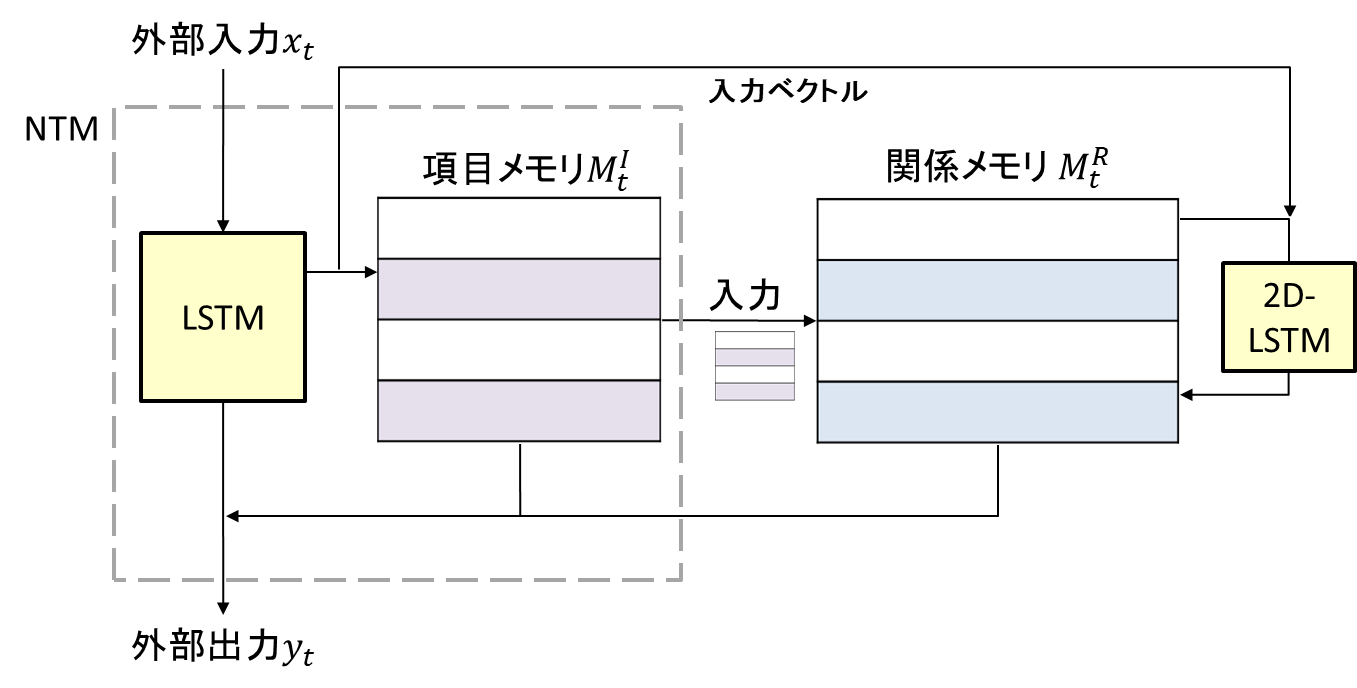
\includegraphics[width=\linewidth]{./figure/img_slide/teian_net.png}
	\caption{提案ネットワーク}
	\label{fig:teian_net}
\end{figure}

ネットワークの構造は大きく3つのモジュールに分けられる。
1つ目は入力の保存・忘却・読み出しを行う項目メモリ$M^I_t$とそのオペレータ。
2つ目は項目メモリの項目間の関係推論を行い、計算した関係情報を保存する関係メモリ$M^R_t$とそのオペレータ。
3つ目は項目メモリの内容を関係メモリに入力する前に項目メモリの項目間順序を整理する順序整理モジュールである。
ネットワークはコントローラLSTMからの出力$o^I_t$、項目メモリからの読み出しベクトル$r^I_t$、関係メモリからの読み出しベクトル$r^R_t$を結合したのちlogistic sigmoid活性化を行い最終的な出力とする。

項目メモリには2.1節で導入したNTMを用いる。関係メモリには2.2節で導入したRMCに変更を加えたものを利用し、この変更は3.1節で説明する。3.2節では新しく提案する順序整理モジュールを2種類説明する。

\section{提案ネットワーク中の関係メモリ}
RMCに変更を加え、項目メモリの各項目間の関係情報を保存する関係メモリとして提案ネットワークに実装する。
提案ネットワーク中の関係メモリは図\ref{fig:teian_rmc}に示すようになる。
時間tにおける関係情報の計算のために、式\ref{eq:rmc_mtil}における入力$x_t$とメモリ$M^R_t$にまたがるアテンションを項目メモリ$M^I_t$と関係メモリ$M^R_t$の連結に対するアテンションに拡張する。
変更後は式\ref{eq:teian_mtil}が示すようにして$\tilde{M}$が計算される。
\begin{equation} \label{eq:teian_mtil}
	\tilde{M} =softmax ( \frac{M_{t-1}W_q ([M_{t-1};M^I_t]W_k)^T}{ \sqrt{d_k}} ) [M_{t-1};M^I_t]W_v
\end{equation}
また$M^R_{t-1}$の更新時には、入力$x_t$の代わりに項目メモリへの書き込みベクトル$w^w_t$を利用する。
従って式\ref{eq:rmc_l2}-\ref{eq:rmc_l4}は式\ref{eq:teian_l2}-\ref{eq:teian_l4}のように変更される。
\begin{equation}\label{eq:teian_l2}
	f_{i,t}=W^f w^w_t +U^f h_{i,t-1}+b^f
\end{equation}
\begin{equation}\label{eq:teian_l3}
	i_{i,t}=W^i w^w_t +U^i h_{i,t-1}+b^i
\end{equation}
\begin{equation}\label{eq:teian_l4}
	o_{i,t}=W^o w^w_t +U^o h_{i,t-1}+b^o 
\end{equation}

\begin{figure}[t]
	\centering
	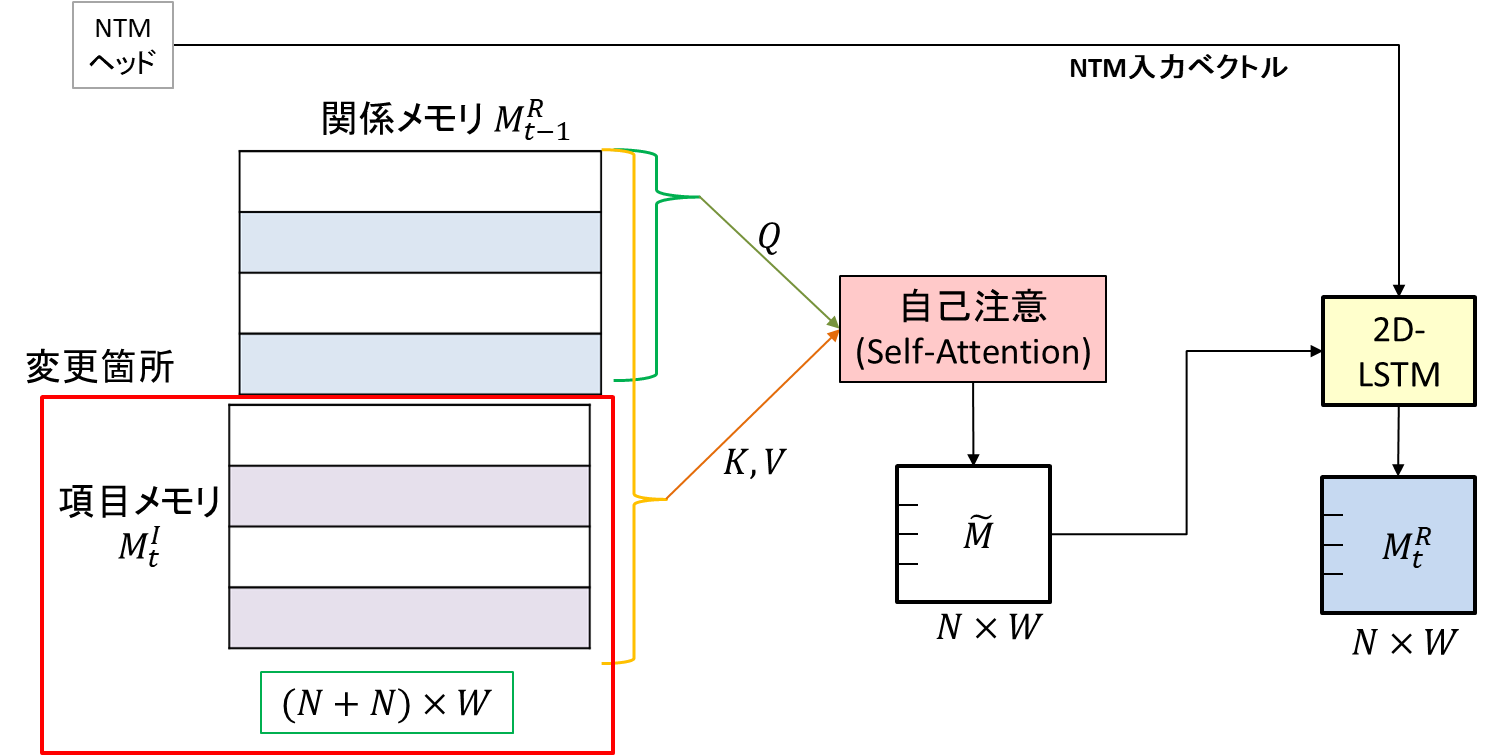
\includegraphics[width=\linewidth]{./figure/img_slide/teian_rmc.png}
	\caption{提案ネットワーク中の関係メモリ}
	\label{fig:teian_rmc}
\end{figure}

\section{順序整理モジュール}
3.2節では項目メモリの順序を解釈・整理する2種類の機構を説明する。3.1節で述べた拡張により、NTMのメモリを関係メモリへの入力とすることが可能となる。
しかしこの実装では項目メモリにおける忘却や上書きは関係メモリの更新と独立して実行されるため、関係メモリへの入力の一貫性が損なわれる問題が予想される。そこで項目メモリを整理し一貫性を持った入力を生成する順序整理モジュールを提案する。

\subsection{書き込み頻度ソート}
項目メモリのヘッドによるメモリの忘却・上書きを疑似的に読み取る手段として、書き込み頻度によるソートを提案する。
時間tにおける各行の書き込み頻度$q_t$($N^I$次元ベクトル)は、式\ref{eq:sum_freq}が示すように$t=1\sim t$での書き込み重みの総和とする。
\begin{equation}\label{eq:sum_freq}
	q_t =\sum_t w^w_t
\end{equation}
関係メモリは式\ref{eq:teian_mtil}において$M^I_t$の代わりに$q_t$に基づいてソートされた$M^I_t$を入力として受け取る。

\subsection{時間リンク行列を利用したグラフアテンション}
DNC\cite{dnc}では各ステップの内容を保存するだけでなく、入力系列内での前後関係の情報を保存するために時間リンク行列を実装している。
時間リンク行列 $L_t$は式\ref{eq:L0}-\ref{eq:L}によって示されるように、時間的に隣接する書き込み重みのouter productionを保存する。
\begin{equation}\label{eq:L0}
	L_0[i,j] =0 \forall i,j
\end{equation}
\begin{equation}\label{eq:Ltii}
	L_t[i,i] =0 \forall i
\end{equation}
\begin{equation}\label{eq:L}
	L_t[i,j] =(1-w^w_t[i]-w^w_t[j])L_{t-1}[i,j]+w^w_t[i]p_{t-1}[j]
\end{equation}
第一項は項目の上書きが発生した時、その位置のリンクをリセットするための項である。
$p_t$は式\ref{eq:prec0},\ref{eq:prec}のようにして計算される。
\begin{equation}\label{eq:prec0}
	p_0 =\boldsymbol{0}
\end{equation}
\begin{equation}\label{eq:prec}
	p_t =(1-\sigma_iw^w_t[i]) p_{t-1}+w^w_t
\end{equation}
提案モジュールでは時間リンク行列を各行が時間的に隣接する程度を表現するグラフと解釈して、グラフアテンション(GAT)\cite{gat}による各項目の変換を試みる。
これにより関係メモリに入力される各項目の特徴量に時間的な順序情報が内包されることが期待できる。
グラフアテンションによる解釈は各行の位置を変更しないため、2.4.1節の書き込み頻度ソートと併用できる。


